\chapter[BPSK Generation and Demodulation]{BPSK Generation and Demodulation}

\section*{Aim}
To set-up and implement circuits to carry out Binary Phase Shift Keying (BPSK). To design demodulating circuits to detect the message from BPSK modulated wave.
\section*{Theory}

Binary Phase Shift Keying is an efficient digital modulation technique and is used for high bit rate data. In this method the phase of unit energy sinusoidal carrier is switched by $180°$ depending upon the input binary sequence. 
\noindent
Let us assume the carrier is represented as: $s(t) = A cos(2\pi f_ct)$.
\noindent
`$A$' represents the peak value of sinusoidal carrier. For a unit ohmic load, the power dissipated would be $P_s = \frac{1}{2A^2}$


\noindent
$ s_1(t) = \sqrt{2P_s} cos (2\pi f_ct) $, to transmit a symbol '1'.
\noindent
To transmit a symbol '0' the signal $ s_2(t) = \sqrt{2P_s} cos (2\pi f_ct + \pi) $ is transmitted. Because $cos (\Theta+\pi) = -cos (\Theta)$, the second equation may be written as $ s_2(t) = - \sqrt{2P_s} cos (2\pi f_ct) $

Combining the above concepts, the BPSK symbol may be represented as:

\begin{equation*}
s(t)= b(t)  \sqrt{2P_s} cos (2\pi f_ct) 
\end{equation*}


where b(t) = +1, when binary 1 is transmitted
b(t)= -1, when binary 0 is transmitted.

The set of modulation and demodulation waveforms are shown in Figure \ref{bpsk-waveforms}.

\begin{figure}[h]
	\centering
	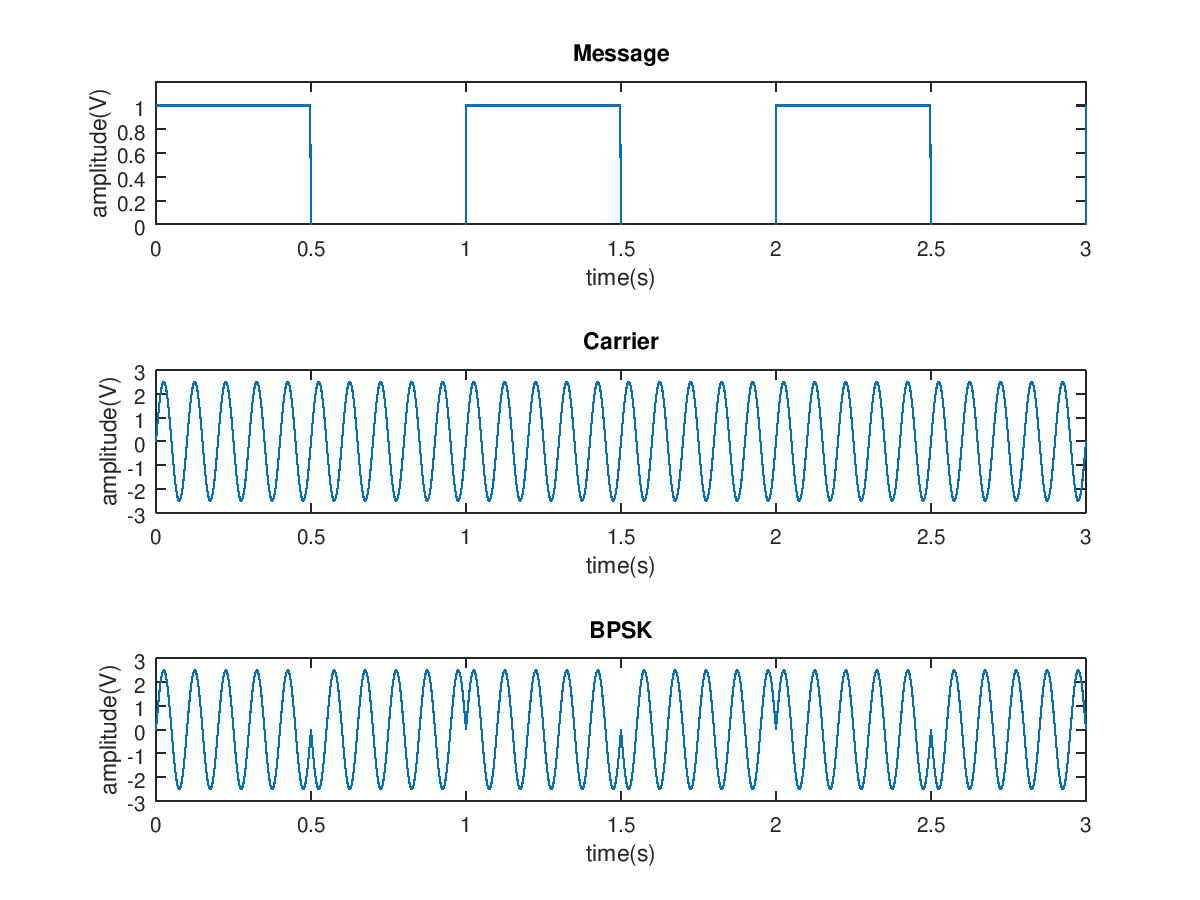
\includegraphics[width=0.8\textwidth]{bpskwaves.png}
	\caption{BPSK Modulator sample waveforms}
	\label{bpsk-waveforms}
\end{figure}


\section*{Design}
\subsection*{BPSK Generation}

A sinusoidal signal and its $180°$ phase shifted versions will act as the carriers for binary data 1 and 0 respectively. A simple inverting amplifier usig Opamp can generate the phase shifted version of the carrier obtained from function generator. For this use $R_f =R_i = 10 k \Omega$.

The binary data can be used as a control signal for switching IC circuits. The binary sequency switches the sinusoidal carrier to output, at the same time the inverted binary sequence switches the phase shifted carrier to output. The two outputs are combined at the load resistor $R_L =1 k\Omega$. See Figure \ref{bpsk-gen} for modulation circuit.


\subsection*{BPSK Demodulation}

A summing amplifier combines the BPSK output and the original carrier to discard the carrier components during the '0' transitions of binary data. This output is similar to BASK signal. It can be demodulated by the step followed in BASK demodulation.

\noindent Use 0A79 diode and $1 k\Omega $ resistor for rectification.
\noindent Use a simple RC lowpass filter to pass the low frequency binary message. Assuming the message frequency is less than $1.5 kHz$,
 
\begin{equation}
f_H=\frac{1}{2\pi R_dC_d}
\end{equation}
\begin{equation}
1.5\ kHz=\frac{1}{2\pi R_dC_d}
\end{equation}
\noindent Select $C_d=\ 0.1 \mu F$. Then $R_d=\ 1.5k\Omega$.
Choose $R_d=\ 1k\Omega$ standard resistor value.\\

The resulting sequency may not be a perfect binary square wave. It can be transformed to a perfect binary sequence by using a threshold detector. The threshold level may adjusted using a $5 k\Omega$ pot.

\section*{Circuit Diagram}

The BASK generation using analog switching IC 4046 is shown in Figure \ref{bpsk-gen} and demodulation using envelop detection technique is shown in Figure \ref{bpsk-det}.

\begin{figure}[h]
	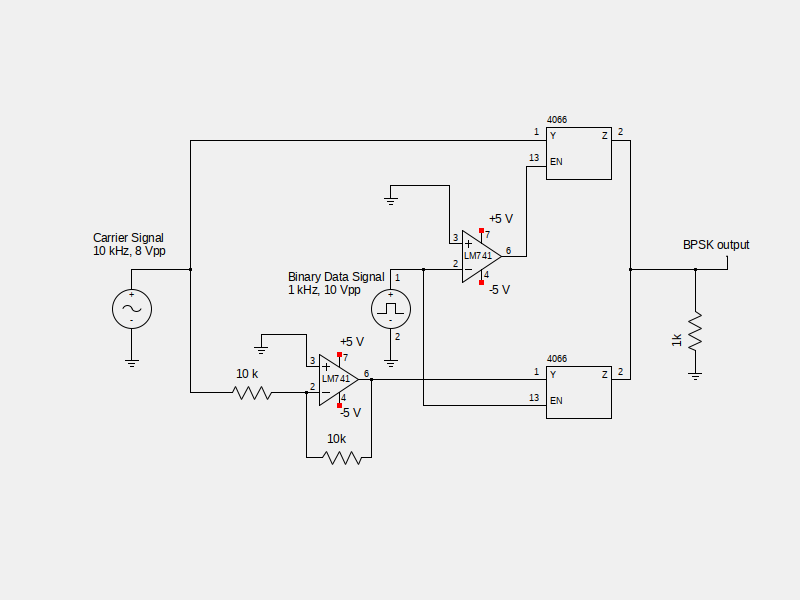
\includegraphics[width=0.8\textwidth]{bpsk.png}
	\caption{BPSK Modulator}
	\label{bpsk-gen}
\end{figure}

\begin{figure}
	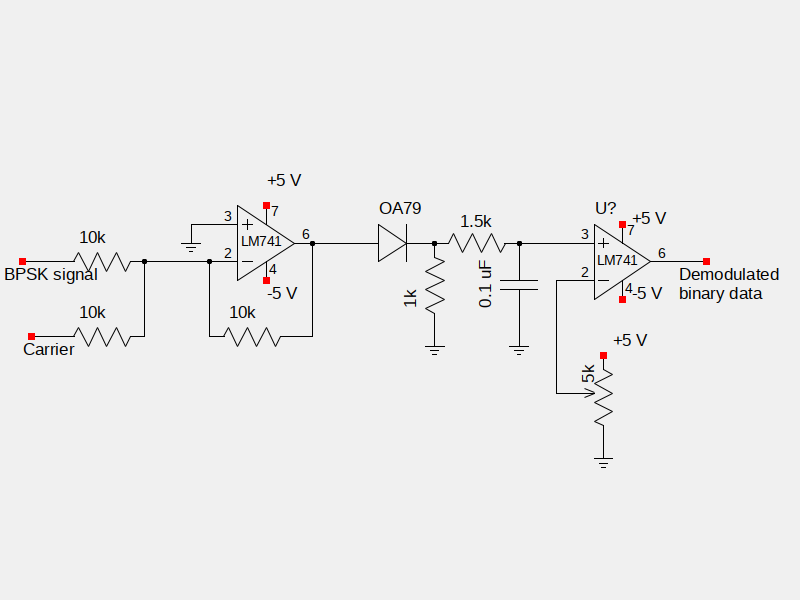
\includegraphics[width=0.8\textwidth, ]{bpsk-demod.png}
	\caption{BPSK Demodulation Circuit}
	\label{bpsk-det}
\end{figure}

\clearpage
\section*{Procedure}
\begin{itemize}
\item
Connect the BPSK generating circuit as shown in the circuit diagram, Figure \ref{bpsk-gen}.
\item
Feed the binary message data ($10 V_{pp}, 1 kHz$ square wave) and the carrier waveform  ($8 V_{pp}, 10 kHz$ sine wave) from the function generator.
\item
Observe the output on a CRO and plot the graphs of the input and output waveforms.
\item
Make the demodulating circuit as shown in the circuit diagram, Figure \ref{bpsk-det}.
\item
Observe the input and output waveforms from BPSK demodulator.
\item 
Obtain the output of demodulator and the control input simultaneously, take the measurements and plot the waveforms.

\end{itemize}
\section*{Observation}
Plot the graphs of input and output waveforms as observed on a CRO.
\section*{Result}

Implemented the BPSK generation and demodulation circuits.